\begin{itemize}
    \item Zusammenfassung der Resultate
    \item Hier geben Sie wieder, was aus der Arbeit als Ergebnis resultiert. Es ist darauf zu achten, dass keine Bewertung der Daten vorweggenommen wird. Diese soll im Diskussionsteil erfolgen. Trotzdem sind die Daten und Resultate mit genügend Text zu erklären. Absolut zentral ist dabei eine präzise, treffende sprachliche Ausdrucksweise. Von Alltagsslang und vagen Ausdrücken ist unbedingt abzusehen. Bei grossen Datenmengen müssen die Rohdaten nicht zwingend publiziert werden.
    \item In Resultate Kapitel, Vergleich erste Algorithmen und Versuche: erste Überlegungen und Tests, alter path planner zhaw, dann densify und interpolate, rrt max hamburg, komplexer algo à la ultimate und dann jetzige implementation, zuerst was hat eth mit mpcc, dann global racetrajectory von tumftm
\end{itemize}

This chapter provides the results of the different approaches that have been used during the evaluation phase. First, the results of the Exploration Algorithm are presented. The test cases were all done visually using Python plots as described in section \ref{sec:Visual Verification with Plots}. Second, the results of the Optimization Algorithm are presented. Again, the test cases are outputted visually using Python plots as described in section \ref{sec:Visual Verification with Plots}. Additionally, each track's calculation times and estimated lap times were calculated. In the end, the integration tests with both algorithms are presented using the Simulation Tool.

\section{Exploration Algorithm}
The exploration algorithm tests were done using Python plots. Track information like cone positions and the starting position of the car were loaded from the track files by the \acrlong{tum}. \cite{tumftm_optimization_algoritm}

\subsection{Acceleration Track} \label{sec:Results Acceleration Track}
Figure \ref{fig:Result Acceleration First Approaches} shows the first approach (a) and the second (b) approach side by side on the acceleration track, which was described in section \ref{sec:Dynamic Events}. The second approach calculated the middle points between the grouped four points used for the triangulation. In addition to the added points, a line was drawn to smoothen the track. Since the plot on (a) and (b) do not plot the start and the end cones (orange cones), they were just used as a basis for the final, more usable algorithm implementation seen in figure \ref{fig:Result Acceleration Final}.
\begin{figure}[H]
    \centering
    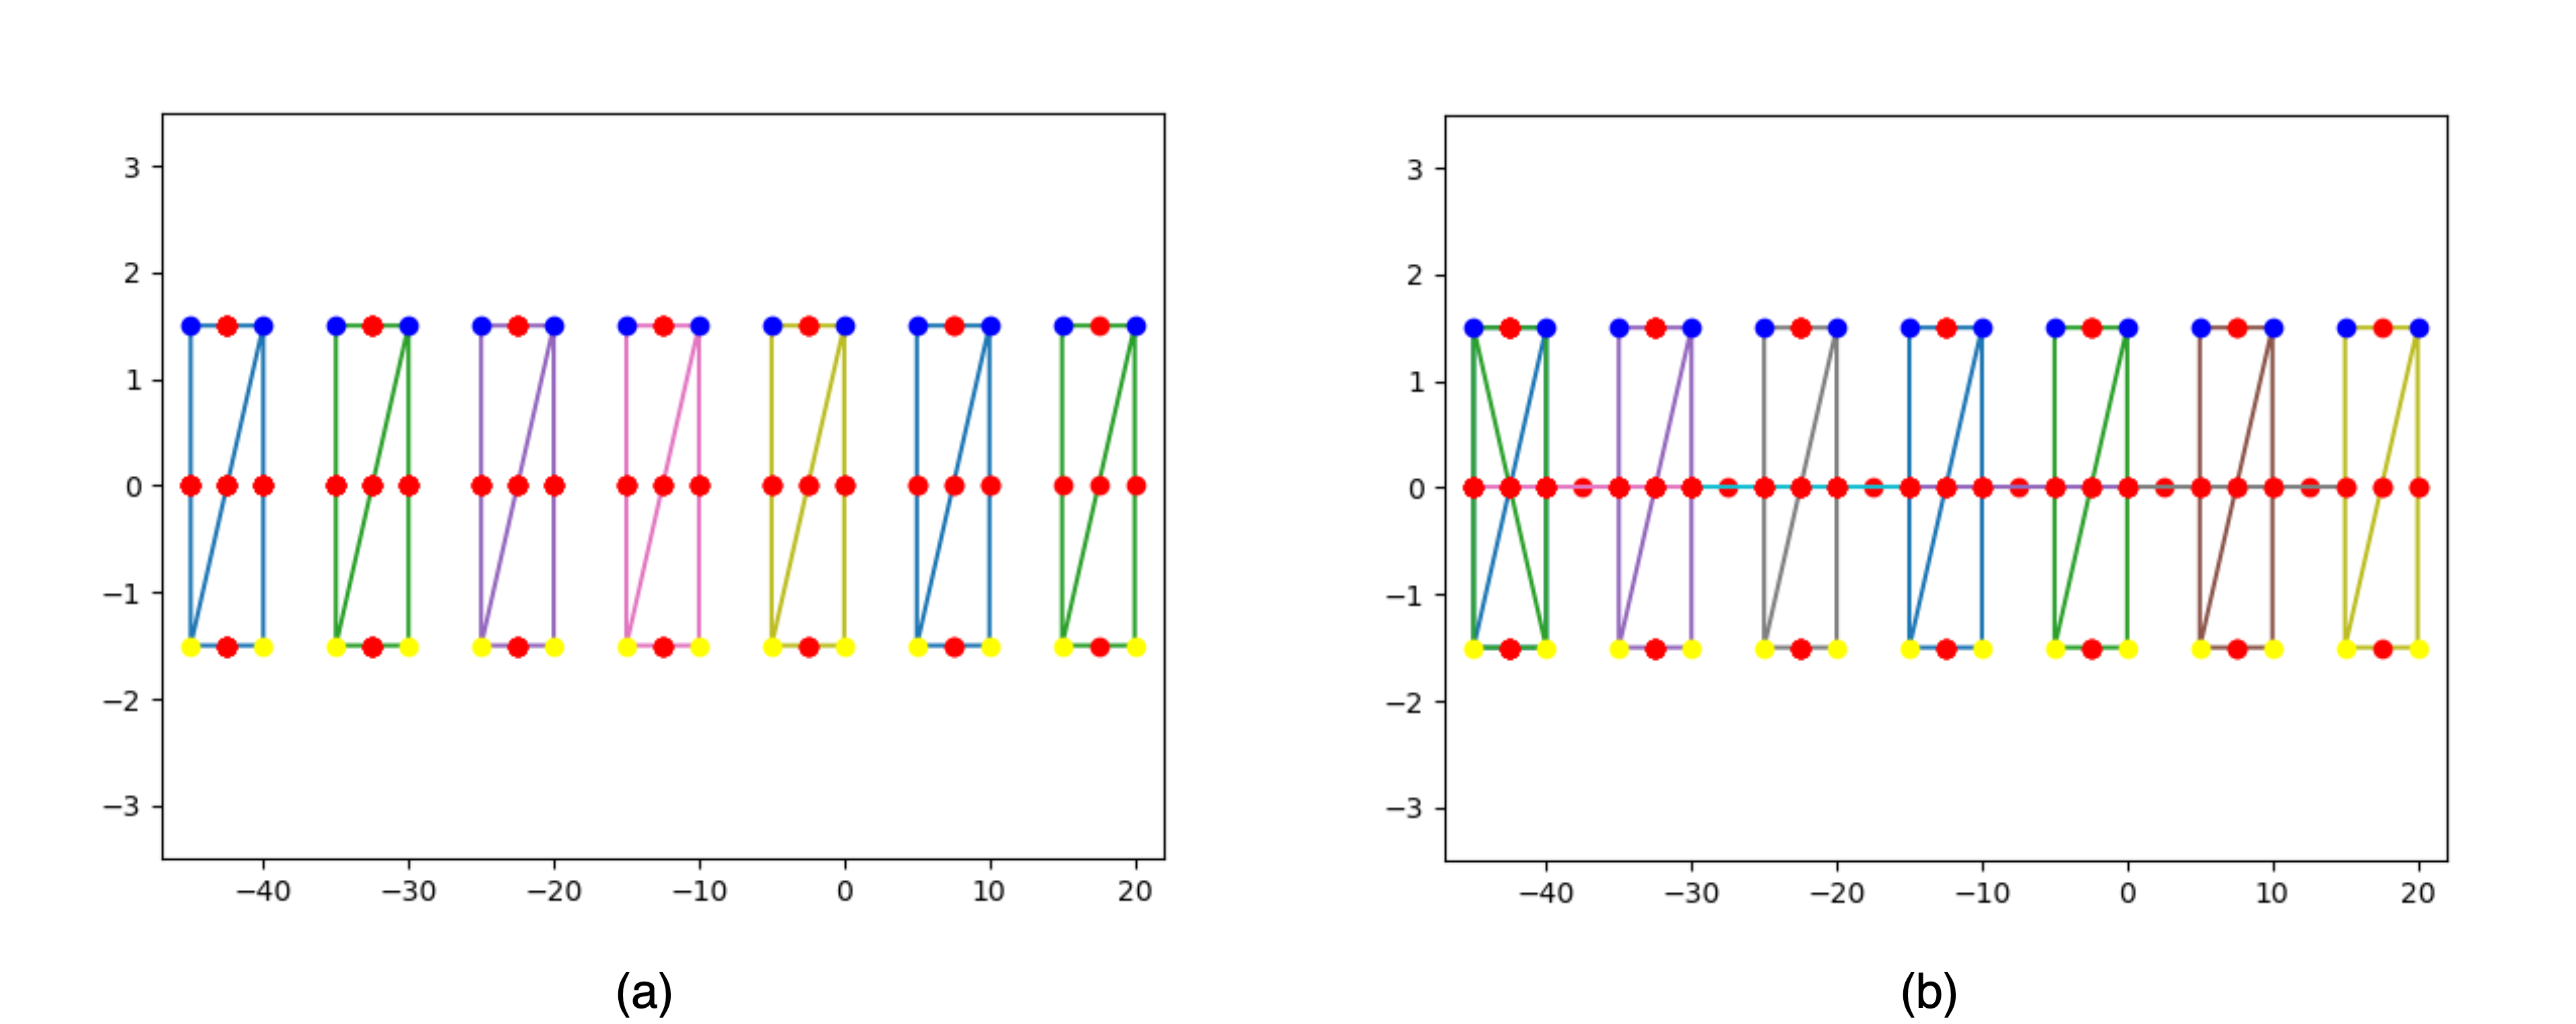
\includegraphics[width=\columnwidth]{Result_Acceleration_First_Approaches.png}
    \caption{Image (a) shows the first approach on the acceleration track, while image (b) shows the second while drawing a middle line.}
    \label{fig:Result Acceleration First Approaches}
\end{figure}
\begin{figure}[H]
    \centering
    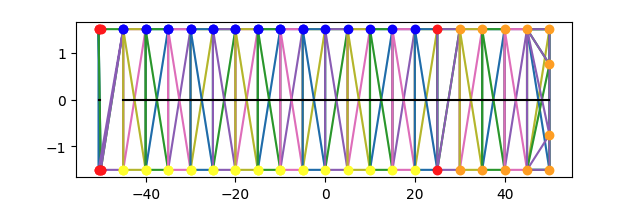
\includegraphics[width=\columnwidth]{Result_Acceleration_final.png}
    \caption{The image shows the final approach on the Acceleration track.}
    \label{fig:Result Acceleration Final}
\end{figure}

\subsection{Small Track} \label{sec:Results Small Track}
The second track that was used for comparison is one of the \acrlong{tum} team, which is called ``Small Track''. \cite{tumftm_optimization_algoritm} This track helped to get an understanding of how the algorithm works on corners with fewer cones on the inner side than on the outer side. Figure \ref{fig:Result Small Track First Approaches} shows a progression of the improvements of the first implementation of the algorithm (a) to the second improved version (b) and the final version of the algorithm in figure \ref{fig:Result Small Track Final}. Again for the first and the second approach, the implementation of publishing the start and end cones (orange cones) was not made already.
\begin{figure}[H]
    \centering
    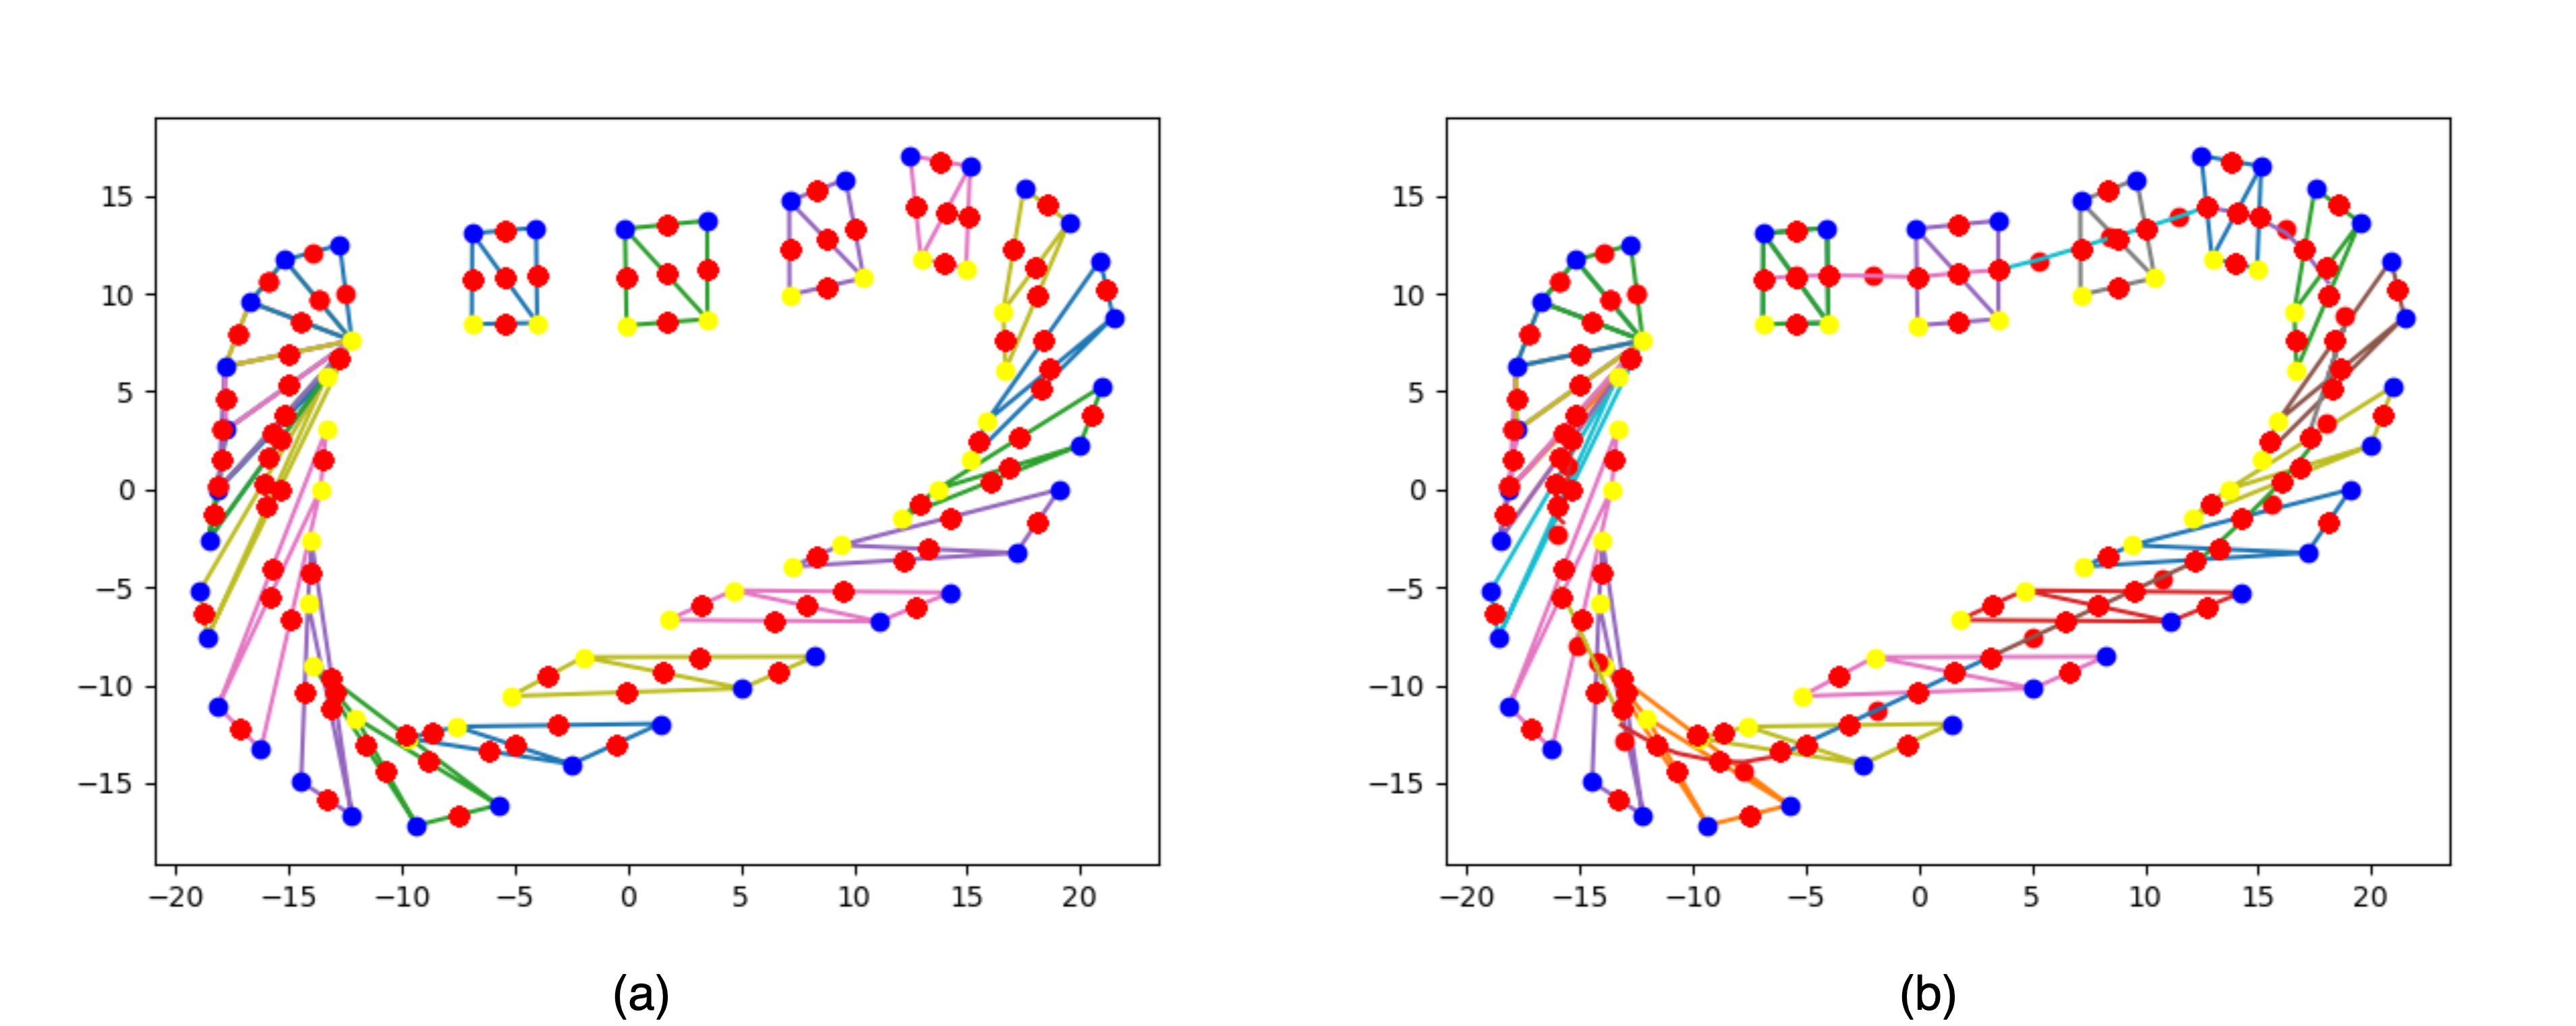
\includegraphics[width=\columnwidth]{Result_SmallTrack_First_Approaches.png}
    \caption{The progression of the improvements of the first implementation (a) to the second implementation (b) is shown.}
    \label{fig:Result Small Track First Approaches}
\end{figure}
\begin{figure}[H]
    \centering
    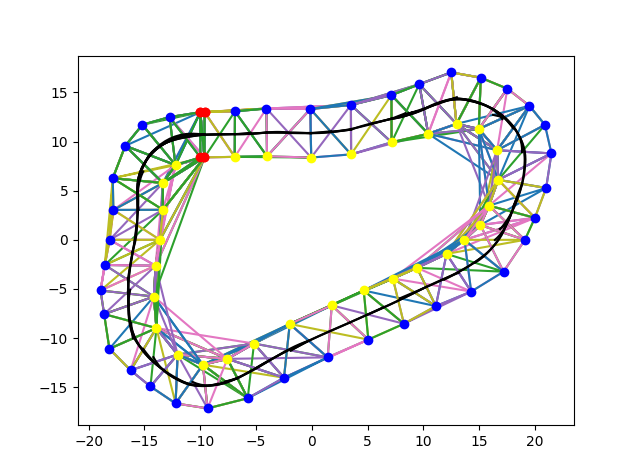
\includegraphics[width=\columnwidth]{Result_SmallTrack_final.png}
    \caption{The image shows the final approach on the Small Track.}
    \label{fig:Result Small Track Final}
\end{figure}

\subsection{Rand Track} \label{sec:Results Rand Track}
The next track, which is shown in figure \ref{fig:Result Rand Final} that was used for testing the final implementation, was the ``Rand'' track. It has more cones and curvature than the ``Small Track'' and shows an example of a track that could have been used for the Track Drive event in the competition, as described in section \ref{sec:Dynamic Events}.
\begin{figure}[H]
    \centering
    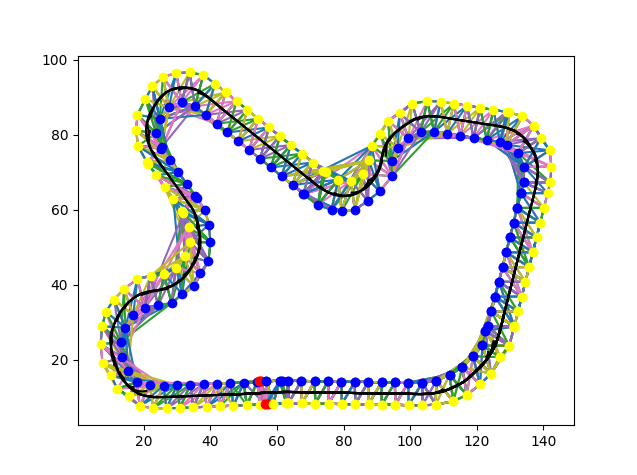
\includegraphics[width=\columnwidth]{Result_Rand_final.png}
    \caption{The ``Rand'' track with the final algorithm implementation.}
    \label{fig:Result Rand Final}
\end{figure}

\subsection{Competition 2021 Track} \label{sec:Results Competition 2021 Track}
Furthermore, a track which was used for a competition in 2021 is shown in figure \ref{fig:Result Comp 2021 Final} with the applied final exploration algorithm. The track consists of more corners than the ``Rand'' track.
\begin{figure}[H]
    \centering
    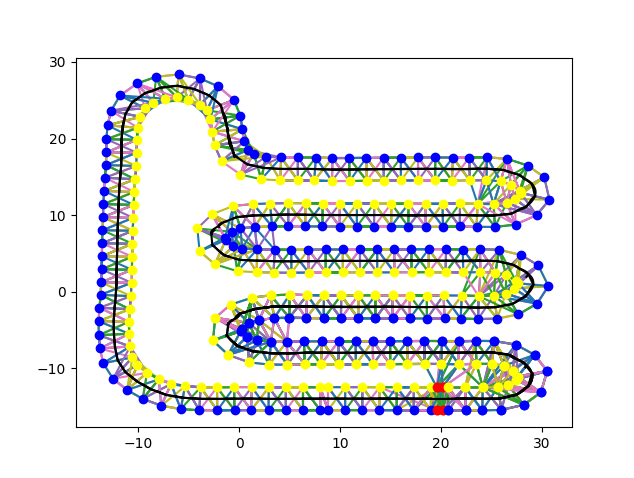
\includegraphics[width=\columnwidth]{Result_Comp2021_final.png}
    \caption{The result of the final exploration algorithm applied on the competition track of 2021.}
    \label{fig:Result Comp 2021 Final}
\end{figure}

\subsection{Garden Light Track} \label{sec:Results Garden Light Track}
Another track used for testing the final implementation was the ``Garden Light'' track. The track has some parts where the left track limits (blue cones) are very close. Additionally, the track has additional cones on its curves. The final result on this track can be seen in figure \ref{fig:Result Garden Light Final}.
\begin{figure}[H]
    \centering
    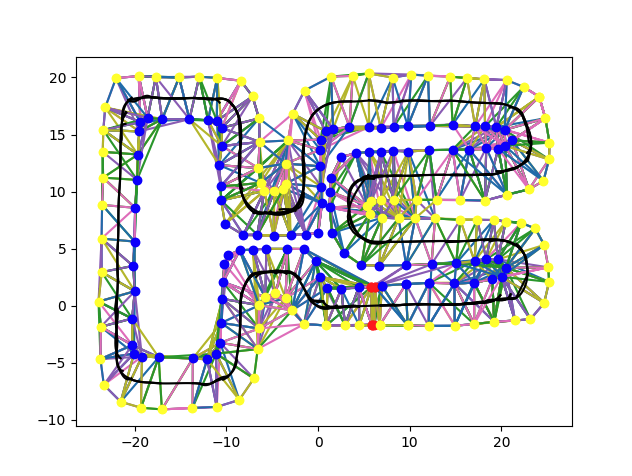
\includegraphics[width=\columnwidth]{Result_GardenLight_final.png}
    \caption{The result of the final exploration algorithm applied on the ``Garden Light`` track.}
    \label{fig:Result Garden Light Final}
\end{figure}

\subsection{Skidpad Track} \label{sec:Results Skidpad Track}
The last example in figure \ref{fig:Result Skidpad Final} shows that the algorithm can also be applied on the ``Skidpad'' track.
\begin{figure}[H]
    \centering
    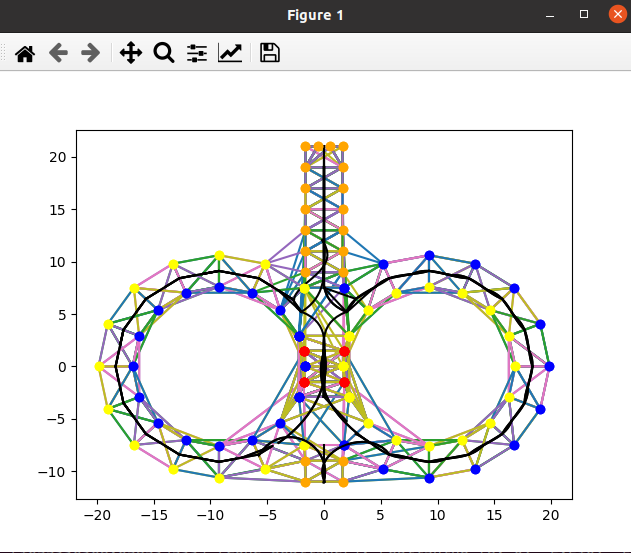
\includegraphics[width=\columnwidth]{Result_Skidpad_final.png}
    \caption{The calculation of the middle line with the Skidpad track.}
    \label{fig:Result Skidpad Final}
\end{figure}

\section{Optimization Algorithm}
\begin{itemize}
    \item verschiedene Screenshot
    \item Zeiten auswertung / vergleich / übersicht
\end{itemize}
ggv
# v_mps,ax_max_mps2,ay_max_mps2
0.0,12.0,12.0
4.0,12.0,12.0
8.0,12.0,12.0
12.0,12.0,12.0
16.0,12.0,12.0
20.0,12.0,12.0
24.0,12.0,12.0
28.0,12.0,12.0
32.0,12.0,12.0
36.0,12.0,12.0
40.0,12.0,12.0
44.0,12.0,12.0
48.0,12.0,12.0
52.0,12.0,12.0
56.0,12.0,12.0
60.0,12.0,12.0
66.0,12.0,12.0
72.0,12.0,12.0

ax machines
# v_mps,ax_max_machines_mps2
0.0,5.3
4.0,5.3
8.0,5.3
12.0,5.3
16.0,5.3
20.0,5.3
24.0,5.3
28.0,5.3
32.0,5.3
36.0,5.3
40.0,5.1
44.0,5.0
48.0,4.6
52.0,4.1
56.0,3.7
60.0,2.7
66.0,2.2
72.0,1.5

calc options

veh_params
"v_max": 30.61,
"length": 2.931,
"width": 1.663,
"mass": 255.0,
"dragcoeff": 0.3,
"curvlim": 0.33,
"g": 9.81
width opt 2.6

cones of track
Exploration:
time of exploration cycle
min max avg nrs total
reference points
Optimization:
mincurv laps 1 2 3

Small Track:
Blue Cones: 37
Yellow Cones: 30
Orange Cones: 0
Big Orange Cones: 4
Unknown Cones: 0
Exploration:
time of exploration cycle
0.0000s 0.0066s 0.0028s 71cycles 0.1974s
865 reference points
Optimization:
mincurv laps 1 2 3 5 8
reference points
Runtime 0.04s 0.08s 0.12s 0.22s 0.48s
lap time 9.17s 18.48s 28.24s 47.39s 78.44s
points 52 102 152 253 404
shortest 0.07s 20.60s 99p
iqp 0.10s 17.88s 102p

Rand:
Blue Cones: 99
Yellow Cones: 109
Orange Cones: 0
Big Orange Cones: 4
Unknown Cones: 0
Exploration:
time of exploration cycle
0.0000s 0.0072s 0.0031s 215cycles 0.6730s
2635 reference points
Optimization:
mincurv laps 1 2 3 5 8
reference points
Runtime 0.12s 0.37s 0.92s 3.41s 13.18s
lap time 24.76s 49.83s 75.69s 129.65s 219.83s
points 194 388 581 967 1546
shortest 0.28s 60.84s 376p
iqp 0.82s 47.80s 384p

Comp 2021:
Blue Cones: 156
Yellow Cones: 156
Orange Cones: 0
Big Orange Cones: 4
Unknown Cones: 1
Exploration:
time of exploration cycle
0.0000s 0.0069s 0.0021s 320cycles 0.6621s
3425 reference points
Optimization:
mincurv laps 1 2 3 5 8
reference points
Runtime 0.12s 0.30s 0.57s 1.66s 5.37s
lap time 29.37s 58.87s 90.06s 146.97s 234.88s
points 130 259 386 642 1029
shortest 0.25s 59.29s 248p
iqp DNF


Garden Light:
Blue Cones: 101
Yellow Cones: 99
Orange Cones: 0
Big Orange Cones: 4
Unknown Cones: 1
Exploration:
time of exploration cycle
0.0000s 0.0076s 0.0029s 205cycles 0.5926s
2631 reference points
Optimization:
mincurv laps 1 2 3 5 8
reference points
Runtime 0.07s 0.17s 0.29s 0.74s 2.03s
lap time 25.20s 48.72s 71.59s 117.31s 190.31s
points 88 173 258 428 682
shortest 0.15s 47.39s 159p
iqp DNF

All 2 Laps
Berlin 2018:
mincurv 38.30s 186.15s 2325p
shortest 23.03s 196.57s 2272p
iqp 102.86s 184.00s 2322p

Modena 2019:
mincurv 26.00s 171.20s 1998p
shortest 14.51s 184.03s 1946p
iqp 69.75s 169.11s 1998p

Handling Track:
mincurv 1.72s 71.94s 582p
shortest 1.15s 74.79s 563p
iqp 3.59s 67.95s 587

Rounded Rectangle:
mincurv 0.39s 36.18s 310p
shortest 0.32s 38.39s 293p
iqp 0.59s 31.28s 303p

Optimization times for berlin\_2018
shortest\_path = 16.72s
Estimated lap time: 89.12s
mincurv = 44.40s
Estimated lap time: 82.46s
mincurv\_iqp = 127.69s
Estimated lap time: 81.06s
mintime = 92.00s
Estimated lap time: 85.77s

\section{Integration}
\begin{itemize}
    \item Test im Python Plots
    \item Simulationstool (Screenshot, evtl. folge von Screenshots), welche strecke (grafik simulationstool)
\end{itemize}

